\section{Visualizing Time and History}\label{sec:vistime}
\begin{comment}
\begin{itemize*}
  \item Visions of history from the past
  \item Correlated pasts
  \item Non-linear scales
  \item Dynamic/interactive timelines
\end{itemize*}
\end{comment}
\epigraph{What does history look like?  How do you draw time?}{\citet[p. 10]{RosenbergGrafton:2010}}
The questions in this quotation from \emph{Cartographies of Time: A History of the Timeline} \citep{RosenbergGrafton:2010}
introduce an important topic in the history of data visualization: how to visualize this history?
Time provides one obvious dimension, but what else can be included to show the details of a history in a static display
or allow users to see more using dynamic and interactive displays?

We have also provided an annotated visual gallery of some timeline designs and visual histories
in our Data Visualization Gallery at \url{datavis.ca/gallery/timelines.php}. The topics covered
include early visual histories, encyclopedic charts, special purpose charts, correlated histories
showing events in one domain in the context of events in other areas, non-linear scales for
time and space as well as dynamic, interactive timelines.  Here we just consider a few fresh examples.

\subsection{The first timelines, reconsidered}
Although there are earlier precursors, the first timelines of modern design---
a horizontal, linear axis for time and vertical positions for place, theme or category of events---
were produced in the mid 1700s, most notably Jacques Barbeau-Doubourg's 1753
\emph{Carte chronologique} and Joseph Priestley's 1765 \emph{Chart of Biography}.

Priestley first published a small ``Specimen'' of this chart as a proof-of-concept,
showing the lifespan of famous men in the years 600 BC to 0 AD, classified as
``statesmen'' (Solon,  $\dots$, Julius Caesar) and ``men of learning'' (Pythagoras, $\dots$, Ovid).
In the same year he published the detailed version \citep{Priestley:1765}
 that quickly became the most popular
and influential timeline of the \Cent{19} and for many years to come.  It showed the
lifespans of more than 2000 people from 1200 BC to 1750 AD, classified by their areas
of achievement (statesmen \& warriors, mathematicians \& physicians, artists \& poets, $\dots$).

\begin{figure}[!htb]
  \centering
  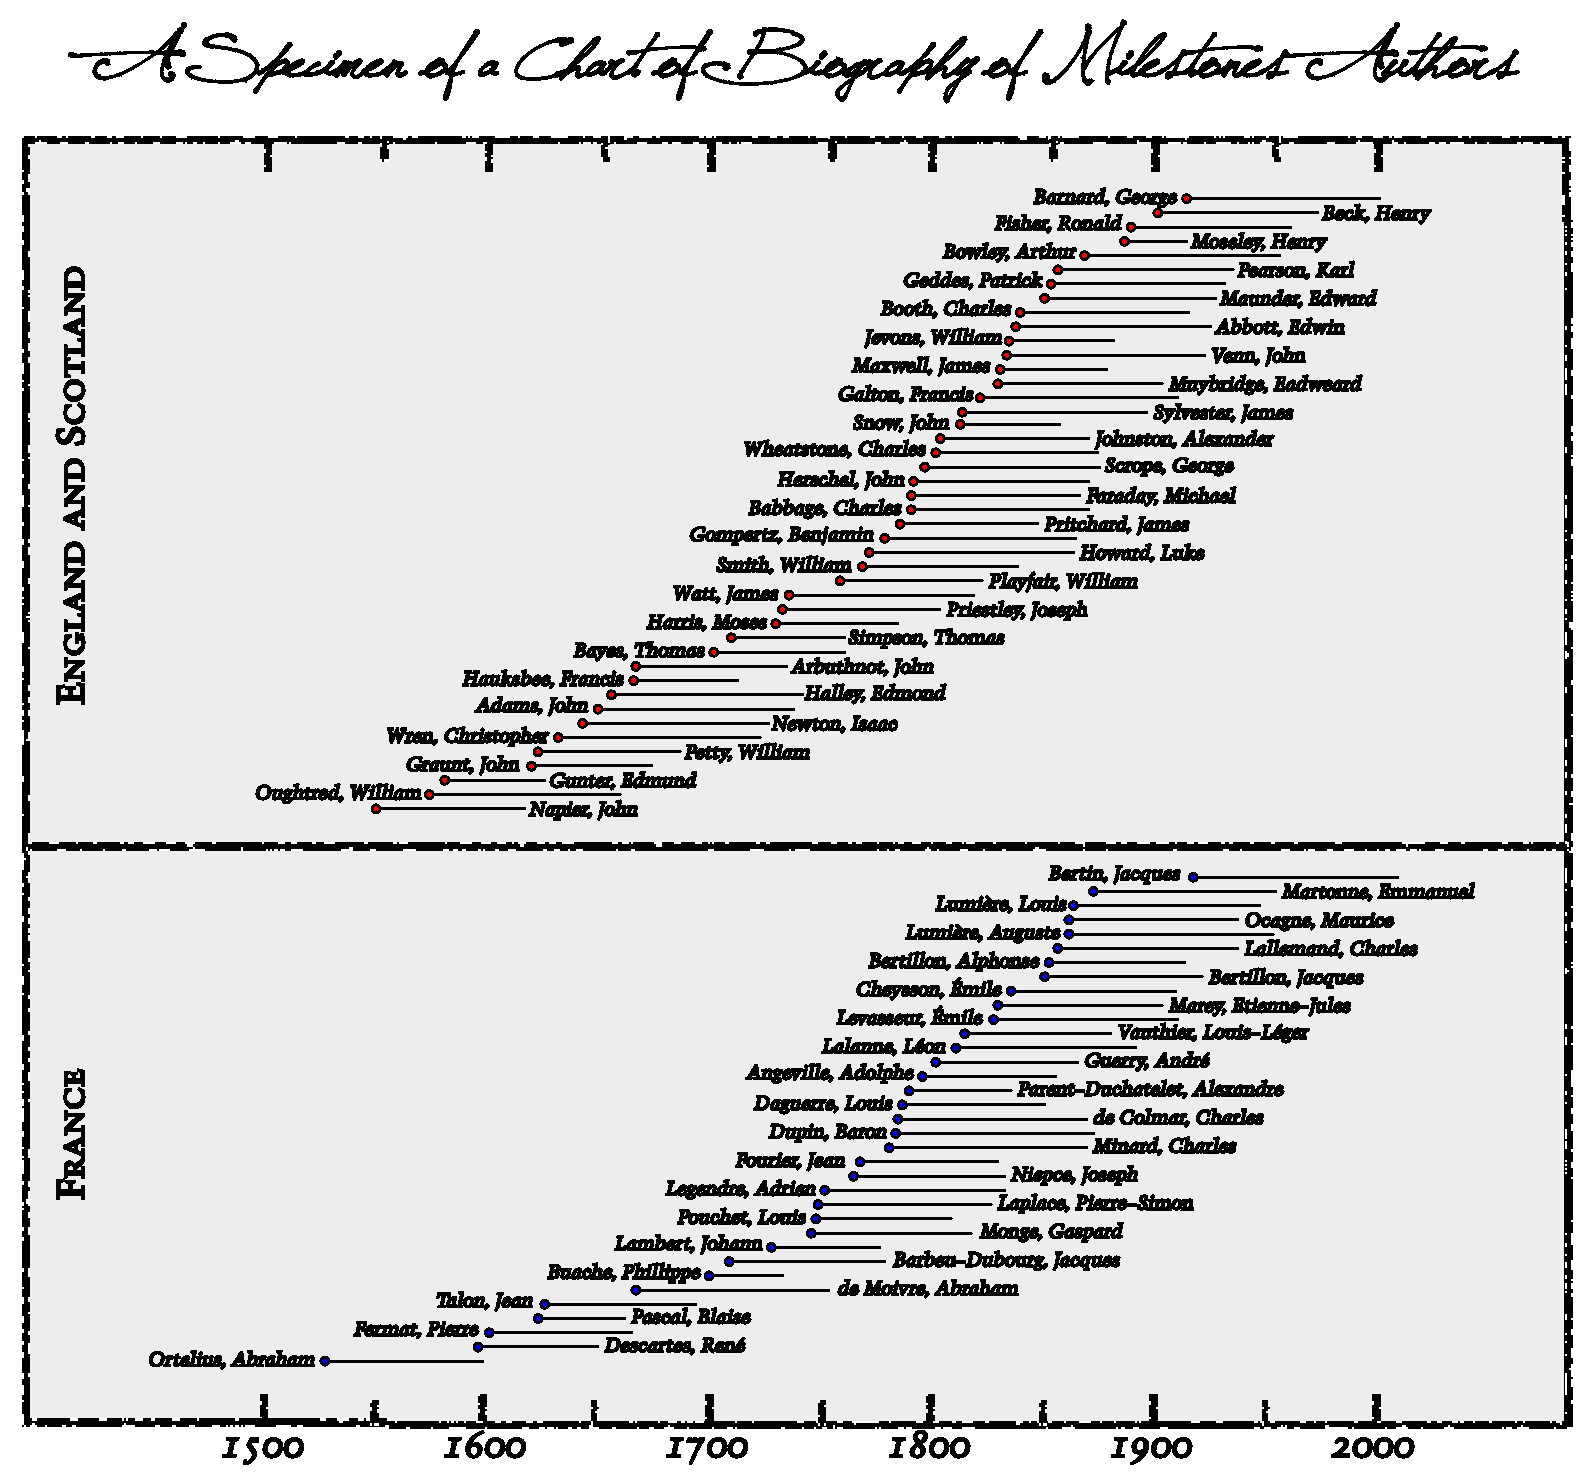
\includegraphics[width=.85\textwidth,clip]{fig/timespan}
  \caption{A modern re-design of Priestley's 1765 \emph{Chart of Biography},
  using information on authors in the Milestones database born in France or the
  United Kindgom. Authors are sorted within country by year of birth and labeled
  alternately at birth and death years, allowing both better lookup and visual
  comparison.
  }
  \label{fig:timespan}
\end{figure}

Priestly's timeline charts can be seen on our Data Visualization Gallery, and we don't reproduce
them here.  Instead we show (\figref{fig:timespan}) a re-design, in his style, of the lifespans
of 79 authors from the Milestones database who were born in France or the United Kindgom between
1500 and 2000. 

\citet[p. 117]{RosenbergGrafton:2010} call Priestley's charts ``masterpieces of visual economy.''
Indeed, they were at the time.  However, in his charts, the famous people were arranged 
haphazardly within category groups, so it is difficult to find specific individuals, 
and nearly impossible to see any trends, over time, or across categories. 

In our version, authors are sorted by birth year within each country and the names are printed
alternately at the year of birth and death. The result, which resembles a cumulative distribution
plot: (a) allows easier visual lookup of names, (b) provides an overall ``lifespan envelope,''
and (c) highlights a few individuals who lived conspicously shorter or longer than their
contemporaries (e.g. shorter: Willam Jevons,  James Maxwell, John Snow, Phillipe Buache).

Of course, to display lifespan \emph{directly} requires a different kind of plot, but one that
would not have been even thinkable by Priestley in 1765.  We return to this question in
\secref{sec:lifespan} (see \figref{fig:lifespan}).


\subsection{Universal histories}
In addition to unrivaled thematic maps and statistical diagrams, the Golden Age of graphics also
gave rise to a variety of novel attempts to visualize history in a comprehensive manner,
combining parallel, intertwined time-flows, text, illustrations, maps and other visual forms.
Among the most impressive is a series of Synchronological Charts of Universal History
produced by Sebastian Adams between 1871--1885.
The 1881 version is 23 feet long and shows 5,885 years of history, from 4004 B.C. to 1881 A.D.
\citet[p. 172]{RosenbergGrafton:2010} call it ``nineteenth-century America's surpassing achievement in complexity and synthetic power.'' 

\figref{fig:Adams1881} shows just a small portion, but the entire chart can be viewed at
\url{http://www.davidrumsey.com/blog/2012/3/28/timeline-maps}.  Adams used a linear scale for
time, and so you can understand why it took 23 linear feet to include all of recorded history.

\begin{figure}[!htb]
  \centering
  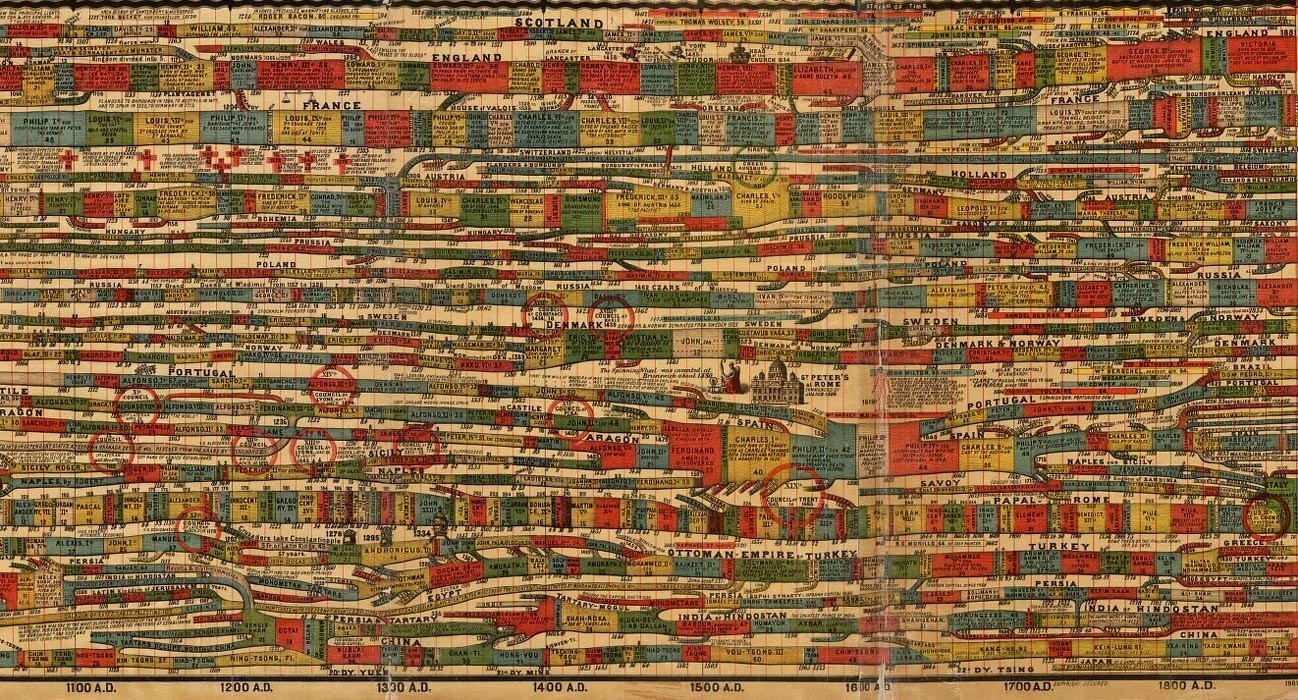
\includegraphics[width=\textwidth,clip]{fig/Adams1881-4}
  \caption{A portion of Sebastian Adams' \emph{Synchronological Chart of Universal History}, 1881,
  covering the \Cent{11}--\Cent{19}.
  }
  \label{fig:Adams1881}
\end{figure}

\subsection{Categorization and non-linear scales}

Linear time scales have the advantage that they
provide uniform resolution and detail across the entire time span, but events in time, or our interest in them are rarely uniformly distributed. Most visual histories are rather sparse at their beginning and very
crowded at their end.
Non-linear scales allow resolution to vary smoothly in some other way, providing for greater detail
in regions of greater interest, most often the recent past.


\begin{figure}[!htb]
  \centering
  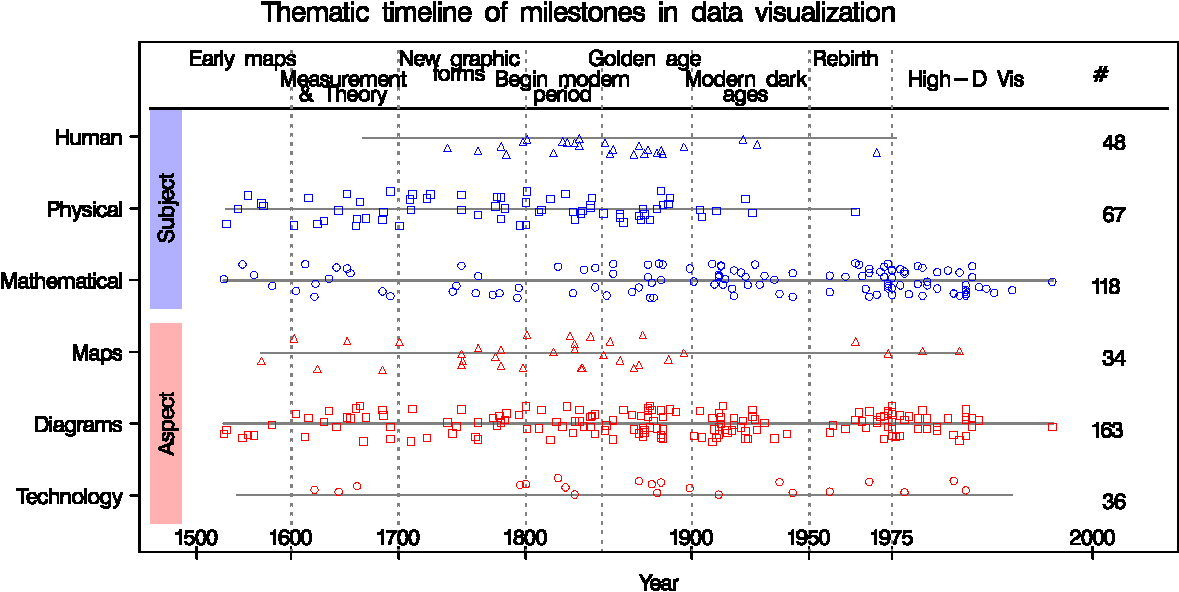
\includegraphics[width=\textwidth,clip]{fig/milecatline}
  \caption{Sketch for a thematic timeline of milestones items, 1500--present,
  categorized by both the Subject (content)
  and Aspect (form) of the milestone item.  To provide greater resolution for more recent events,
  time (Year) is shown on a square-root scale, going backward from the year 2000.
  }
  \label{fig:milecatline}
\end{figure}

\figref{fig:milecatline} is really just a proof-of-concept sketch for something that a graphic artist
could use as a starting point for a chart of
the history of data visualization. It uses the events from the
Milestones Project, categorized by two correlated factors: 
Subject area or content has been
categorized as dealing with human populations, physical properties of the world or
mathematics and statistics; aspect or form has been categorized as dealing with
cartography, graphs and diagrams or technology. 

To provide greater resolution for more recent events, we have used a reverse square-root
scale going backward from the year 2000. Specifically, Year on the horizontal time axis
is actually plotted according to the formula $\textrm{Year}^\star = 2* (25 - \sqrt{(2000 - \textrm{Year})})$,
giving the more pleasing result that the modern period 1800--2000 occupies about 60\% of the scale,
although it comprises only 40\% of the range.

